\documentclass[14pt]{extarticle}
% math symbols
\usepackage{sfg}


\usepackage{amssymb,amsmath}
\synctex=1
% for different compilers
\usepackage{ifpdf}
% geometry of page
\usepackage[margin=2cm]{geometry}

% if pdflatex, then
\ifpdf
\usepackage[russian]{babel}
\usepackage[utf8]{inputenc}
\usepackage[unicode]{hyperref}
\usepackage[pdftex]{graphicx}
\usepackage{cmlgc}
% if xelatex, then
\else
% math fonts
\usepackage{fouriernc}
% xelatex specific packages
\usepackage[xetex]{hyperref}
\usepackage{xltxtra}	% \XeLaTeX macro
\usepackage{xunicode}	% some extra unicode support
\defaultfontfeatures{Mapping=tex-text}
\usepackage{polyglossia}	% instead of babel in xelatex
\usepackage{indentfirst}	% 
\setdefaultlanguage{russian}
% fonts
\newfontfamily\cyrillicfont{SchoolBookC}
\newfontfamily\cyrillicfontsf{TextBookC}
\setmonofont{Consolas}
\fi

% several pictures in one figure
\usepackage{subfig}
% calc in TeX expressions
\usepackage{calc}
% nice pictures and plots
\usepackage{pgfplots,tikz,circuitikz}
% different libraries for pictures
\usetikzlibrary{%
  arrows,%
  calc,%
  patterns,%
  decorations.pathreplacing,%
  decorations.pathmorphing,%
  decorations.markings,%
  intersections,%
  decorations.text%
}

\usepackage{tkz-euclide}

\usepackage{enumitem}
\renewcommand{\theenumi}{(\asbuk{enumi})}
\renewcommand{\labelenumi}{\asbuk{enumi})}
\AddEnumerateCounter{\Asbuk}{\@Asbuk}{\CYRM}
\AddEnumerateCounter{\asbuk}{\@asbuk}{\cyrm}

\begin{document}

\section*{Задача}

\subsection*{Условие}
Угол между двумя зеркалами равен $\varphi$. Луч всета падает на одно из них так, что он образует с ним угол $\varphi_1$. Отразившись в зеркалах два раза, он образует с другим зеркалом угол $\varphi_2$. Можно ли узнать, какой угол состовляют падающий и отраженный лучи?
\subsection*{Векторное Решение}
Пусть $e_1$ и $e_2$ -- векторы нормалей двух зеркал, а $x$ -- единичный вектор, сонаправленный с падающим лучом.
Введем оператор $R_i$ над векторами.
\begin{align*}
R_ir = r - 2 e_i (r e_i)
\end{align*}

Если луч с сонаправленным единичным вектором $r$ падает на плоскость $i$, то он отражается с новым сонаправленным вектором $R_ir$, поскольку $(r e_i)$ -- перпендикулярная зеркалу составляющая r, которая должна изменить знак.\\
Теперь найдем Луч, отразившийся от двух зеркал 	с сонаправленным вектором $x_1$.

\begin{align*}
&x_1 = R_2(R_1x) = (R_1x) - 2 e_i ((R_1x) e_i) = (x - 2 e_i (x e_i)) - 2 e_i ((x - 2 e_i (x e_i)) e_i)=\\
&x - (2e_1x)e_1 + (4(e_1e_2)(xe_1)-2(e_2x))e_2
\end{align*}

Нам надо найти угол между $x$ и $x_1$. Заметим, что по построению \\$|x| = |x_1| = 1$.


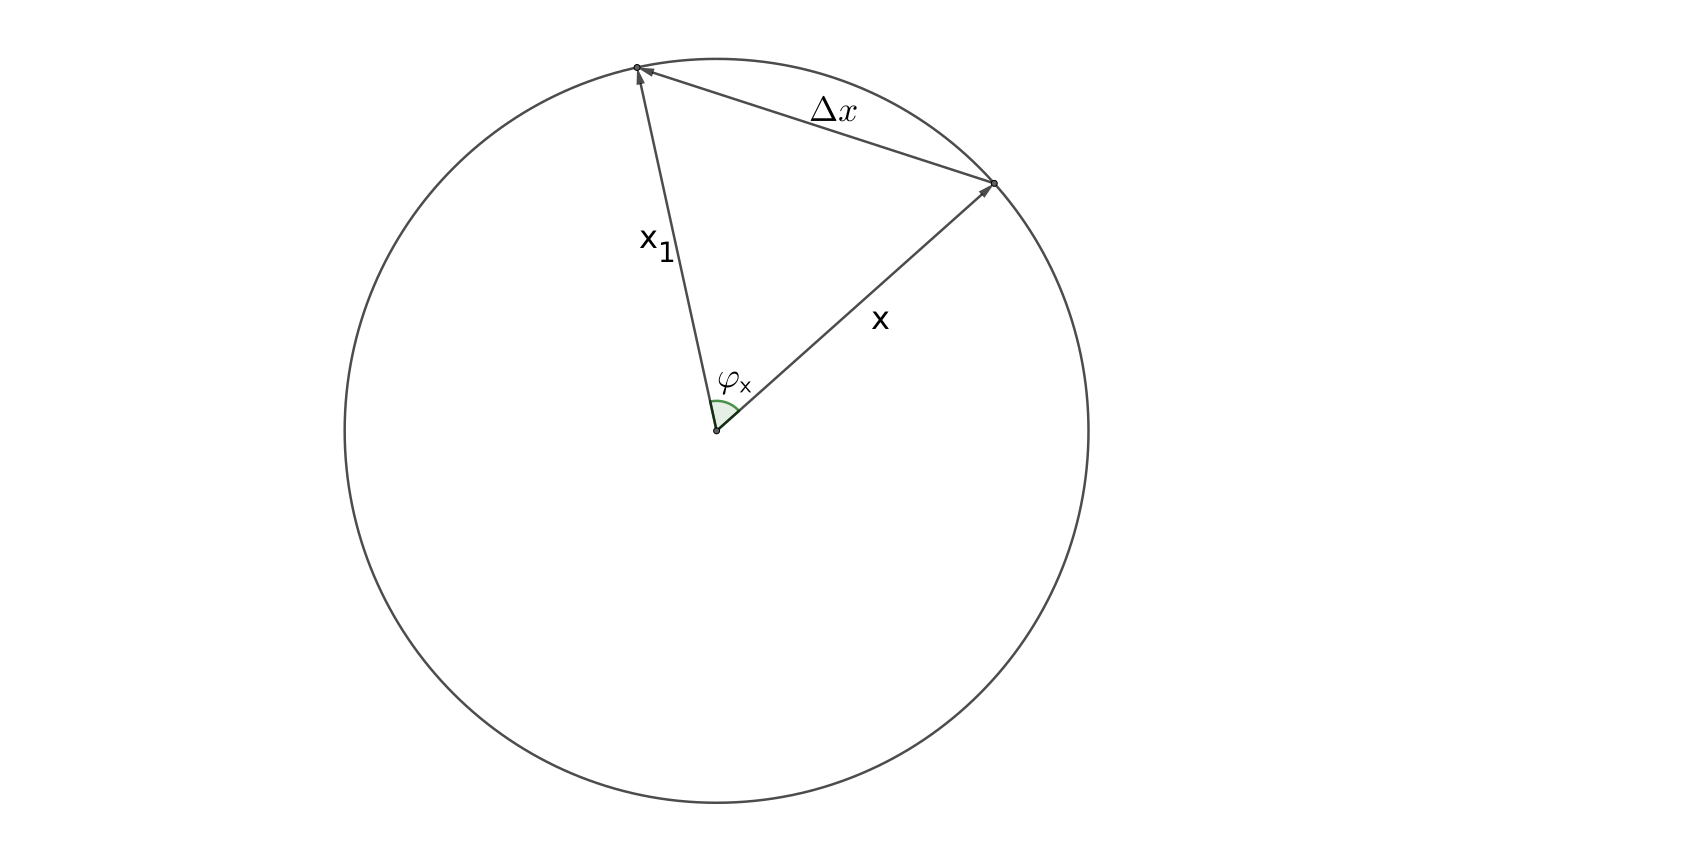
\includegraphics[width=0.7\textwidth]{{./3ch}.png}

Тогда, если $\Delta x = x_1 - x$, то $2sin(\varphi_x / 2) = |\Delta x| / |x| = |\Delta x|$,\\ где $\varphi_x$ -- угол между лучами.

Теперь выразим все скалярные величины через известные углы.
\begin{align*}
&x e_1 = sin(\varphi_1)\\
&x_1 e_2 = sin(\varphi_2)\\
&e_1 e_2 = cos(\varphi)\\
&\Delta x = (4(e_1 e_2)(x e_1) - 2 (e_2 x)) e_2 - (2 x e_1) e_1 = (4 cos(\varphi) sin(\varphi_1) - 2 e_2 x) e_2 - 2 sin(\varphi_1) e_1\\
&sin(\varphi_2) = x_1 e_2 = 4 cos(\varphi) sin(\varphi_1) - 2 e_2 x + e_2 x = 4 cos(\varphi) sin(\varphi_1) - e_2 x \\
&\Delta x = (2sin(\varphi_2) - 4 cos(\varphi) sin(\varphi_1)) e_2 - 2 sin(\varphi_1) e_1
\end{align*}

Осталось только найти модуль $\Delta x$.
\begin{align*}
(\Delta x / 2)^2 = 8 cos^2(\varphi) sin^2(\varphi_1) - 6 cos(\varphi) sin(\varphi_1) sin(\varphi_2) + sin^2(\varphi_1) + sin^2(\varphi_2)
\end{align*}

То есть,
\begin{align*}
\varphi_x = 2 asin(\sqrt{8 cos^2(\varphi) sin^2(\varphi_1) - 6 cos(\varphi) sin(\varphi_1) sin(\varphi_2) + sin^2(\varphi_1) + sin^2(\varphi_2)})
\end{align*}

\includegraphics[height=0.95\textheight]{{./3ch_1}.png}

\end{document}